\documentclass[%
%  reprint,
superscriptaddress,
% groupedaddress,
%unsortedaddress,
% runinaddress,
% frontmatterverbose, 
% preprint,
%preprintnumbers,
%nofootinbib,
%nobibnotes,
%bibnotes,
 amsmath,amssymb,
%aps,
prl,
%pra,
prb,
% rmp,
%prstab,
% prstper,
%floatfix,
]{revtex4-2}


\usepackage{graphicx}% Include figure files
\usepackage{dcolumn}% Align table columns on decimal point
\usepackage{bm}% bold math
\usepackage{blindtext}
\usepackage{float}
\usepackage{caption}
\usepackage{cleveref}
\usepackage{subcaption}
\usepackage{xcolor}

\newcommand{\etal}{{\it et al.}~}
\newcommand{\bom}{\boldsymbol{\omega}}
\newcommand{\hel}{\textsuperscript{4}He }

\def\red#1{\textcolor{red}{#1}}
\def\blue#1{\textcolor{blue}{#1}}
\def\magenta#1{\textcolor{magenta}{#1}}
\newcommand*{\NOTE}[1]{\textbf{\color{red}[#1]}}

\def \s{\mathbf{s}}
\def \v{\mathbf{v}}
\def \x{\mathbf{x}}
\def \r{\mathbf{r}}
\def \k{\mathbf{k}}

\def \cm{\mathrm{cm}}
\def \cms{\mathrm{cm/s}}
\def \sec{\mathrm{s}}
\def \K{\mathrm{K}}

\def\red{\textcolor{red}}


\begin{document}
\preprint{APS/123-QED}

\title{Supplementary Materials: Experimental and theoretical evidence of universality in superfluid vortex
reconnections}

\author{P. Z. Stasiak}
\affiliation{School of Mathematics, Statistics and Physics, Newcastle University, Newcastle upon Tyne, NE1 7RU, United Kingdom}

\author{Y. Xing}
\author{Y. Alihosseini}
\affiliation{National High Magnetic Field Laboratory, 1800 East Paul Dirac Drive, Tallahassee, Florida 32310, USA}
\affiliation{Mechanical Engineering Department, FAMU-FSU College of Engineering, Tallahassee, Florida 32310, USA}


\author{C.F. Barenghi}
\author{A. Baggaley}
\affiliation{School of Mathematics, Statistics and Physics, Newcastle University, Newcastle upon Tyne, NE1 7RU, United Kingdom}

\author{W. Guo}
\affiliation{National High Magnetic Field Laboratory, 1800 East Paul Dirac Drive, Tallahassee, Florida 32310, USA}
\affiliation{Mechanical Engineering Department, FAMU-FSU College of Engineering, Tallahassee, Florida 32310, USA}


\author{L. Galantucci}
\affiliation{Istituto per le Applicazioni del Calcolo ``M. Picone" IAC CNR, Via dei Taurini 19, 00185 Roma, Italy}

\author{G. Krstulovic}
\affiliation{Universit\'e C\^ote d'Azur, Observatoire de la C\^ote d'Azur, CNRS,Laboratoire Lagrangre, Boulevard de l'Observatoire CS 34229 - F 06304 NICE Cedex 4, France}


\maketitle

\section{Experimental Method}

To produce solidified deuterium ($\rm D_2$) tracer particles, we slowly inject a gas mixture of $5\%$ $\rm D_2$ and $95\%$ ${}^{4}\rm He$ into a superfluid helium bath. Our gas injection system is similar to that described by Fonda et al. \cite{fonda2016injection}. A solenoid valve is installed to control the duration of the gas injection, and a needle valve is used to regulate the gas flow rate. The injected $\rm D_2$ gas solidifies into small ice particles with a mean radius of 1.1 $\mu \rm m$, derived from the particle settling velocities in quiescent superfluid helium \cite{tang2023visualization}. A 473 nm continuous-wave laser sheet (thickness: $0.8~\rm mm$) illuminates the particles, and their motion in the laser sheet plane is recorded by a camera at 200 frames per second with a maximum resolution of $2560 \times 1440$ pixels. We then identify vortex reconnection events from the recorded videos, and manually track the coordinates of the trapped particles for the pre- (if captured) and post-reconnection. Knowing the particle coordinates, the minimum distance between the reconnecting vortices $\delta^{\pm}(t)$ can be measured. We calculate the prefactors $A^\pm$ using the slopes of linear fits to the $\delta^2(t)$ data.

\section{Numerical Method}

\begin{figure}
	\centering
	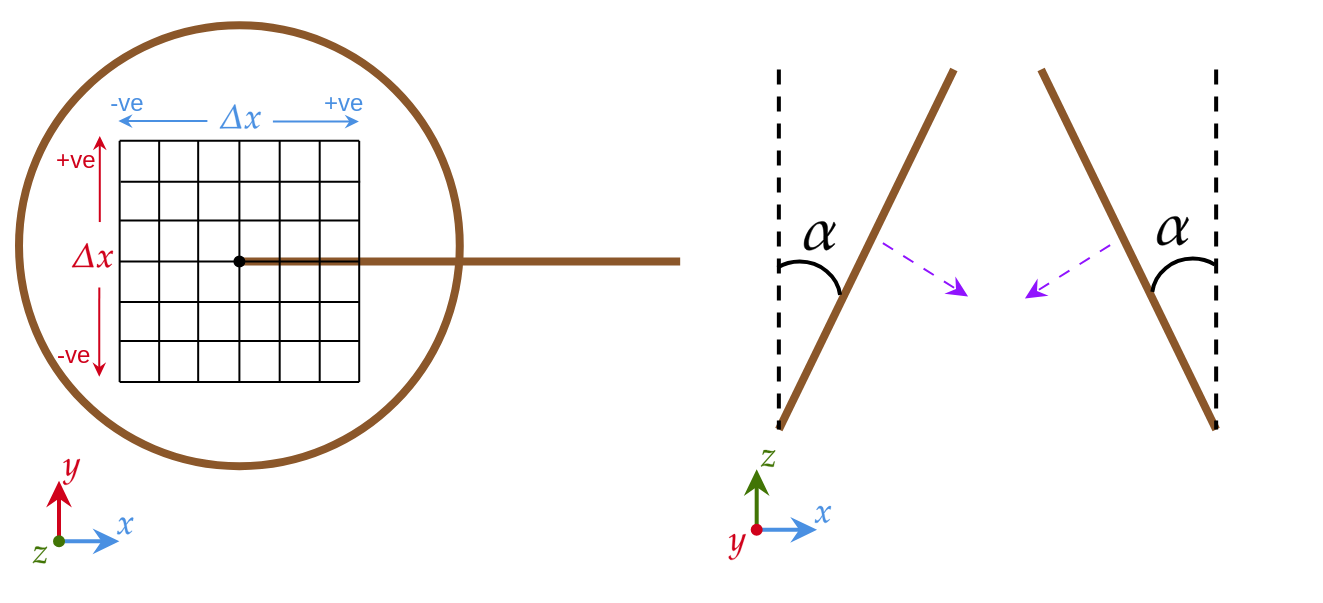
\includegraphics[width=0.9\textwidth]{init-cond-schem.png}
	\caption{Schematic diagram for numeric initial condition. \emph{Left:} Hopf-link. \emph{Right:} Oblique collision.}
	\label{fig: ring-coll-viz}
\end{figure}
Using Schwarz mesoscopic model \cite{schwarzThreedimensionalVortexDynamics1988a}, vortex lines can be described as space curves $\s(\xi,t)$ of infinitesimal thickness, with a single quantum of circulation $\kappa=h/m_4=9.97\times10^{-8}\text{m}^2/\text{s}$, where $h$ is Planck's constant, $m_4=6.65\times10^{-27}\text{kg}$ is the mass of one helium atom, $\xi$ is the natural parameterisation, arclength, and $t$ is time. These conditions are a good approximation, since the vortex core radius of superfluid \textsuperscript{4}He($a_0=10^{-10}\text{m}$) is much smaller than any of the length scale of interest in turbulent flows. The equation of motion is
\begin{equation}
	\dot{\s}(\xi,t) = \v_s + \frac{\beta}{1+\beta}\left[\v_{ns}\cdot \s'\right]\s' + \beta\s'\times\v_{ns}+\beta'\s'\times\left[\s'\times \v_{ns}\right],
\end{equation}
where $\dot{\s}=\partial\s/\partial t$, $\s'=\partial\s/\partial \xi$ is the unit tangent vector, $\v_{ns}=\v_n - \v_s$, $\v_n$ and $\v_s$ are the normal fluid and superfluid velocities at $\s$ and $\beta$,$\beta'$ are temperature and Reynolds number dependent mutual fricition coefficients \cite{galantucciNewSelfconsistentApproach2020b}. The superfluid velocity $\v_s$ at a point $\x$ is determined by the Biot-Savart law
\begin{equation}
	\v_s(\x,t) = \frac{\kappa}{4\pi}\oint_{\mathcal{T}}\frac{\s'(\xi,t)\times\left[\x-\s(\xi,t)\right]}{|\x-\s(\xi,t)|}d\xi,
\end{equation}
where $\mathcal{T}$ represents the entire vortex configuration.
There is currently a lack of a well-defined theory of vortex reconnections in superfluid helium, like for the Gross-Pitaevskii equation \cite{villoisIrreversibleDynamicsVortex2020,villoisUniversalNonuniversalAspects2017a,promentMatchingTheoryCharacterize2020a}. An \emph{ad hoc} vortex reconnection algorithm is employed to resolve the collisions of vortex lines \cite{baggaleySensitivityVortexFilament2012a}.

A \emph{two-way model} is crucial to understand the accurately interept the back-reaction effect of the normal fluid on the vortex line and vice-versa \cite{stasiakCrossComponentEnergyTransfer2024}. We self-consistently evolve the normal fluid $\v_n$ with a modified Navier-Stokes equation
\begin{equation}
	\frac{\partial \v_n}{\partial t} + (\v_n\cdot\nabla)\v_n = -\nabla\frac{p}{\rho} + \nu_n\nabla^2\v_n + \frac{\mathbf{F}_{ns}}{\rho_n},
\end{equation}
\begin{equation}
	\mathbf{F}_{ns} = \oint_{\mathcal{T}}\mathbf{f}_{ns}\delta(\x-\x)d\xi, \quad \nabla\cdot\v_n=0,
\end{equation}
where $\rho=\rho_n + \rho_s$ is the total density, $\rho_n$ and $\rho_s$ are the normal fluid and superfluid densities, $p$ is the pressure, $\nu_n$ is the kinematic viscosity of the normal fluid and $\mathbf{f}_{ns}$ is the local friction per unit length \cite{galantucciCoupledNormalFluid2015a}
\begin{equation}
	\mathbf{f}_{ns} = -D\s'\times\left[\s'\times(\dot{\s}-\v_n)\right]-\rho_n\kappa\s'\times(\v_n-\dot{\s}), 
\end{equation}
where $D$ is a coefficient dependent on the vortex Reynolds number and intrinsic properties of the normal fluid.

The results in this Letter are reported in dimensionless units, where the characteristic length scale is $\tilde{\lambda}=D/D_0$, where $D^3=(1\times10^{-3}\text{m})^3$ is the dimensional cube size, $D_0^3=(2\pi)^3$ is the non-dimensional cubic computational domain. The time scale is given by $\tilde{\tau} = \tilde{\lambda}^2\nu_n^0/\nu_n$, where the non-dimensional viscosity $\nu_n^0$ resolves the small scales of the normal fluid. In these simulations, these quantities are $\tilde{\lambda}=1.59\times10^{-4}\text{cm}$, $\nu_n^0=0.16$ and $\tilde{\tau} = 0.183$s at $T=0K$ and at $T=1.9K$ and $\tilde{\tau}=0.242$s at $T=2.1K$.
We consider two distinct initial vortex geometries at $T=0K,1.9K$ and $2.1K$. The first is a Hopf link, two linked rings of radius $R\approx1$ with an offset in the $xy$-plane defined by parameters $\Delta l_x$ and $\Delta l_y$. The offsets are chosen so that $(\Delta l_x, \Delta l _y) \in \lbrace(0.125i,0.125j)|i,j=-3,\cdots,3 \rbrace$, a total of 49 reconnections for each temperature. The second geometry is a collision of vortex rings of radius $R\approx1$ in a tent-like configuration (see Fig. \ref{fig: ring-coll-viz}), making an angle $\alpha$ with the vertical. We take 12 realisations of $\alpha$, such that $\alpha\in\lbrace i\pi/13|i=1,\cdots,12\rbrace$. 

In both cases, normal fluid rings are initially superimposed to match the vortex lines, eliminating the transient phase of generating normal fluid structures. The Lagrangian discretisation of vortex lines is $\Delta\xi=0.025$ (a total of 668 discretiation points) with a timestep of $\Delta t_{VF}=1.25\times10^{-5}$. A total of $N=256^3$ Eulerian mesh points were used for the normal fluid, with a timestep of $\Delta t_{NS} = 40\Delta t_{VF}$.

%\bibliography{references}% Produces the bibliography via BibTeX.
%apsrev4-2.bst 2019-01-14 (MD) hand-edited version of apsrev4-1.bst
%Control: key (0)
%Control: author (8) initials jnrlst
%Control: editor formatted (1) identically to author
%Control: production of article title (0) allowed
%Control: page (0) single
%Control: year (1) truncated
%Control: production of eprint (0) enabled
\begin{thebibliography}{10}%
\makeatletter
\providecommand \@ifxundefined [1]{%
 \@ifx{#1\undefined}
}%
\providecommand \@ifnum [1]{%
 \ifnum #1\expandafter \@firstoftwo
 \else \expandafter \@secondoftwo
 \fi
}%
\providecommand \@ifx [1]{%
 \ifx #1\expandafter \@firstoftwo
 \else \expandafter \@secondoftwo
 \fi
}%
\providecommand \natexlab [1]{#1}%
\providecommand \enquote  [1]{``#1''}%
\providecommand \bibnamefont  [1]{#1}%
\providecommand \bibfnamefont [1]{#1}%
\providecommand \citenamefont [1]{#1}%
\providecommand \href@noop [0]{\@secondoftwo}%
\providecommand \href [0]{\begingroup \@sanitize@url \@href}%
\providecommand \@href[1]{\@@startlink{#1}\@@href}%
\providecommand \@@href[1]{\endgroup#1\@@endlink}%
\providecommand \@sanitize@url [0]{\catcode `\\12\catcode `\$12\catcode
  `\&12\catcode `\#12\catcode `\^12\catcode `\_12\catcode `\%12\relax}%
\providecommand \@@startlink[1]{}%
\providecommand \@@endlink[0]{}%
\providecommand \url  [0]{\begingroup\@sanitize@url \@url }%
\providecommand \@url [1]{\endgroup\@href {#1}{\urlprefix }}%
\providecommand \urlprefix  [0]{URL }%
\providecommand \Eprint [0]{\href }%
\providecommand \doibase [0]{https://doi.org/}%
\providecommand \selectlanguage [0]{\@gobble}%
\providecommand \bibinfo  [0]{\@secondoftwo}%
\providecommand \bibfield  [0]{\@secondoftwo}%
\providecommand \translation [1]{[#1]}%
\providecommand \BibitemOpen [0]{}%
\providecommand \bibitemStop [0]{}%
\providecommand \bibitemNoStop [0]{.\EOS\space}%
\providecommand \EOS [0]{\spacefactor3000\relax}%
\providecommand \BibitemShut  [1]{\csname bibitem#1\endcsname}%
\let\auto@bib@innerbib\@empty
%</preamble>
\bibitem [{\citenamefont {Fonda}\ \emph {et~al.}(2016)\citenamefont {Fonda},
  \citenamefont {Sreenivasan},\ and\ \citenamefont
  {Lathrop}}]{fonda2016injection}%
  \BibitemOpen
  \bibfield  {author} {\bibinfo {author} {\bibfnamefont {E.}~\bibnamefont
  {Fonda}}, \bibinfo {author} {\bibfnamefont {K.~R.}\ \bibnamefont
  {Sreenivasan}},\ and\ \bibinfo {author} {\bibfnamefont {D.~P.}\ \bibnamefont
  {Lathrop}},\ }\bibfield  {title} {\bibinfo {title} {{Sub-micron solid air
  tracers for quantum vortices and liquid helium flows}},\ }\href
  {https://doi.org/10.1063/1.4941337} {\bibfield  {journal} {\bibinfo
  {journal} {Rev. Sci. Instrum.}\ }\textbf {\bibinfo {volume} {87}},\ \bibinfo
  {pages} {025106} (\bibinfo {year} {2016})}\BibitemShut {NoStop}%
\bibitem [{\citenamefont {Tang}\ \emph {et~al.}(2023)\citenamefont {Tang},
  \citenamefont {Guo}, \citenamefont {Kobayashi}, \citenamefont {Yui},
  \citenamefont {Tsubota},\ and\ \citenamefont
  {Kanai}}]{tang2023visualization}%
  \BibitemOpen
  \bibfield  {author} {\bibinfo {author} {\bibfnamefont {Y.}~\bibnamefont
  {Tang}}, \bibinfo {author} {\bibfnamefont {W.}~\bibnamefont {Guo}}, \bibinfo
  {author} {\bibfnamefont {H.}~\bibnamefont {Kobayashi}}, \bibinfo {author}
  {\bibfnamefont {S.}~\bibnamefont {Yui}}, \bibinfo {author} {\bibfnamefont
  {M.}~\bibnamefont {Tsubota}},\ and\ \bibinfo {author} {\bibfnamefont
  {T.}~\bibnamefont {Kanai}},\ }\bibfield  {title} {\bibinfo {title} {Imaging
  quantized vortex rings in superfluid helium to evaluate quantum
  dissipation},\ }\href@noop {} {\bibfield  {journal} {\bibinfo  {journal}
  {Nat. Commun.}\ }\textbf {\bibinfo {volume} {14}},\ \bibinfo {pages} {2941}
  (\bibinfo {year} {2023})}\BibitemShut {NoStop}%
\bibitem [{\citenamefont
  {Schwarz}(1988)}]{schwarzThreedimensionalVortexDynamics1988a}%
  \BibitemOpen
  \bibfield  {author} {\bibinfo {author} {\bibfnamefont {{\relax
  KW}.}~\bibnamefont {Schwarz}},\ }\bibfield  {title} {\bibinfo {title}
  {Three-dimensional vortex dynamics in superfluid {$^{4}$}{{He}}},\
  }\href@noop {} {\bibfield  {journal} {\bibinfo  {journal} {Phys. Rev. B}\
  }\textbf {\bibinfo {volume} {38}},\ \bibinfo {pages} {2398} (\bibinfo {year}
  {1988})}\BibitemShut {NoStop}%
\bibitem [{\citenamefont {Galantucci}\ \emph {et~al.}(2020)\citenamefont
  {Galantucci}, \citenamefont {Baggaley}, \citenamefont {Barenghi},\ and\
  \citenamefont {Krstulovic}}]{galantucciNewSelfconsistentApproach2020b}%
  \BibitemOpen
  \bibfield  {author} {\bibinfo {author} {\bibfnamefont {L.}~\bibnamefont
  {Galantucci}}, \bibinfo {author} {\bibfnamefont {A.~W.}\ \bibnamefont
  {Baggaley}}, \bibinfo {author} {\bibfnamefont {C.~F.}\ \bibnamefont
  {Barenghi}},\ and\ \bibinfo {author} {\bibfnamefont {G.}~\bibnamefont
  {Krstulovic}},\ }\bibfield  {title} {\bibinfo {title} {A new self-consistent
  approach of quantum turbulence in superfluid helium},\ }\href@noop {}
  {\bibfield  {journal} {\bibinfo  {journal} {Eur. Phys. J. Plus}\ }\textbf
  {\bibinfo {volume} {135}},\ \bibinfo {pages} {547} (\bibinfo {year}
  {2020})}\BibitemShut {NoStop}%
\bibitem [{\citenamefont {Villois}\ \emph {et~al.}(2020)\citenamefont
  {Villois}, \citenamefont {Proment},\ and\ \citenamefont
  {Krstulovic}}]{villoisIrreversibleDynamicsVortex2020}%
  \BibitemOpen
  \bibfield  {author} {\bibinfo {author} {\bibfnamefont {A.}~\bibnamefont
  {Villois}}, \bibinfo {author} {\bibfnamefont {D.}~\bibnamefont {Proment}},\
  and\ \bibinfo {author} {\bibfnamefont {G.}~\bibnamefont {Krstulovic}},\
  }\bibfield  {title} {\bibinfo {title} {Irreversible {{Dynamics}} of {{Vortex
  Reconnections}} in {{Quantum Fluids}}},\ }\href
  {https://doi.org/10.1103/PhysRevLett.125.164501} {\bibfield  {journal}
  {\bibinfo  {journal} {Phys. Rev. Lett.}\ }\textbf {\bibinfo {volume} {125}},\
  \bibinfo {pages} {164501} (\bibinfo {year} {2020})}\BibitemShut {NoStop}%
\bibitem [{\citenamefont {Villois}\ \emph {et~al.}(2017)\citenamefont
  {Villois}, \citenamefont {Proment},\ and\ \citenamefont
  {Krstulovic}}]{villoisUniversalNonuniversalAspects2017a}%
  \BibitemOpen
  \bibfield  {author} {\bibinfo {author} {\bibfnamefont {A.}~\bibnamefont
  {Villois}}, \bibinfo {author} {\bibfnamefont {D.}~\bibnamefont {Proment}},\
  and\ \bibinfo {author} {\bibfnamefont {G.}~\bibnamefont {Krstulovic}},\
  }\bibfield  {title} {\bibinfo {title} {Universal and nonuniversal aspects of
  vortex reconnections in superfluids},\ }\href
  {https://doi.org/10.1103/PhysRevFluids.2.044701} {\bibfield  {journal}
  {\bibinfo  {journal} {Phys. Rev. Fluids}\ }\textbf {\bibinfo {volume} {2}},\
  \bibinfo {pages} {044701} (\bibinfo {year} {2017})}\BibitemShut {NoStop}%
\bibitem [{\citenamefont {Proment}\ and\ \citenamefont
  {Krstulovic}(2020)}]{promentMatchingTheoryCharacterize2020a}%
  \BibitemOpen
  \bibfield  {author} {\bibinfo {author} {\bibfnamefont {D.}~\bibnamefont
  {Proment}}\ and\ \bibinfo {author} {\bibfnamefont {G.}~\bibnamefont
  {Krstulovic}},\ }\bibfield  {title} {\bibinfo {title} {Matching theory to
  characterize sound emission during vortex reconnection in quantum fluids},\
  }\href {https://doi.org/10.1103/PhysRevFluids.5.104701} {\bibfield  {journal}
  {\bibinfo  {journal} {Phys. Rev. Fluids}\ }\textbf {\bibinfo {volume} {5}},\
  \bibinfo {pages} {104701} (\bibinfo {year} {2020})}\BibitemShut {NoStop}%
\bibitem [{\citenamefont
  {Baggaley}(2012)}]{baggaleySensitivityVortexFilament2012a}%
  \BibitemOpen
  \bibfield  {author} {\bibinfo {author} {\bibfnamefont {A.~W.}\ \bibnamefont
  {Baggaley}},\ }\bibfield  {title} {\bibinfo {title} {The sensitivity of the
  vortex filament method to different reconnection models},\ }\href@noop {}
  {\bibfield  {journal} {\bibinfo  {journal} {J. Low Temp. Phys.}\ }\textbf
  {\bibinfo {volume} {168}},\ \bibinfo {pages} {18} (\bibinfo {year}
  {2012})}\BibitemShut {NoStop}%
\bibitem [{\citenamefont {Stasiak}\ \emph {et~al.}(2024)\citenamefont
  {Stasiak}, \citenamefont {Baggaley}, \citenamefont {Krstulovic},
  \citenamefont {Barenghi},\ and\ \citenamefont
  {Galantucci}}]{stasiakCrossComponentEnergyTransfer2024}%
  \BibitemOpen
  \bibfield  {author} {\bibinfo {author} {\bibfnamefont {P.~Z.}\ \bibnamefont
  {Stasiak}}, \bibinfo {author} {\bibfnamefont {A.~W.}\ \bibnamefont
  {Baggaley}}, \bibinfo {author} {\bibfnamefont {G.}~\bibnamefont
  {Krstulovic}}, \bibinfo {author} {\bibfnamefont {C.~F.}\ \bibnamefont
  {Barenghi}},\ and\ \bibinfo {author} {\bibfnamefont {L.}~\bibnamefont
  {Galantucci}},\ }\bibfield  {title} {\bibinfo {title} {Cross-{{Component
  Energy Transfer}} in {{Superfluid Helium-4}}},\ }\bibfield  {journal}
  {\bibinfo  {journal} {J. Low Temp. Phys.}\ }\href
  {https://doi.org/10.1007/s10909-023-03042-5} {10.1007/s10909-023-03042-5}
  (\bibinfo {year} {2024})\BibitemShut {NoStop}%
\bibitem [{\citenamefont {Galantucci}\ \emph {et~al.}(2015)\citenamefont
  {Galantucci}, \citenamefont {Sciacca},\ and\ \citenamefont
  {Barenghi}}]{galantucciCoupledNormalFluid2015a}%
  \BibitemOpen
  \bibfield  {author} {\bibinfo {author} {\bibfnamefont {L.}~\bibnamefont
  {Galantucci}}, \bibinfo {author} {\bibfnamefont {M.}~\bibnamefont
  {Sciacca}},\ and\ \bibinfo {author} {\bibfnamefont {{\relax
  CF}.}~\bibnamefont {Barenghi}},\ }\bibfield  {title} {\bibinfo {title}
  {Coupled normal fluid and superfluid profiles of turbulent helium {{II}} in
  channels},\ }\href@noop {} {\bibfield  {journal} {\bibinfo  {journal} {Phys.
  Rev. B}\ }\textbf {\bibinfo {volume} {92}},\ \bibinfo {pages} {174530}
  (\bibinfo {year} {2015})}\BibitemShut {NoStop}%
\end{thebibliography}%


\end{document}
